\begin{figure}[H]
  \centering
  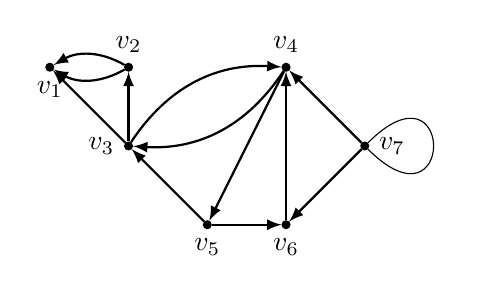
\begin{tikzpicture}[every loop/.style={}]
      \tikzset{enclosed/.style={draw, circle, inner sep=0pt, minimum size=.10cm, fill=black}}
    \node[enclosed] at (1,2) (v_2) [label=above:\(v_2\)] {};
    \node[enclosed] at (3,2) (v_4) [label=above:\(v_4\)] {};
    \node[enclosed] at (4,1) (v_7) [label=right:\(v_7\)] {};
    \node[enclosed] at (2,0) (v_5) [label=below:\(v_5\)] {};
    \node[enclosed] at (3,0) (v_6) [label=below:\(v_6\)] {};
    \node[enclosed] at (1,1) (v_3) [label=left:\(v_3\)] {};
    \node[enclosed] at (0,2) (v_1) [label=below:\(v_1\)] {};

    \footnotesize
    	\path[->, > = latex, thick] (v_2) edge[bend right] node {} (v_1);
    	\path[->, > = latex, thick] (v_2) edge[bend left] node {} (v_1);
    	\path[->, > = latex, thick] (v_3) edge[bend left] node {} (v_4);
    	\path[->, > = latex, thick] (v_3) edge node {} (v_2);
    	\path[->, > = latex, thick] (v_4) edge[bend left] node {} (v_3);
    	\path[->, > = latex, thick] (v_4) edge node {} (v_5);
   		\path[->, > = latex, thick] (v_6) edge node {} (v_4);
		\path[->, > = latex, thick] (v_7) edge node {} (v_4);
		\path[->, > = latex, thick] (v_7) edge node {} (v_6);
		\path[->, > = latex, thick] (v_5) edge node {} (v_6);
		\path[->, > = latex, thick] (v_5) edge node {} (v_3);
		\path[->, > = latex, thick] (v_3) edge node {} (v_1);
		\path (v_7) edge [out=315,in=45,looseness=50] node {} (v_7);




  \end{tikzpicture}
  \caption{Orienteret multigraf.}
  \label{fig:orienteretmulti}
\end{figure}

\begin{table} [H]

	\centering
	\begin{tabular}{ |p{3cm}|p{3cm}|}
 		\hline
 		Knuder & Naboknuder\\
 		\hline
 		$v_1$ & \\
		$v_2$ & $v_1$ \\
		$v_3$ & $v_1$, $v_2$, $v_4$ \\
		$v_4$ & $v_3$, $v_5$, \\
		$v_5$ & $v_3$, $v_6$ \\
		$v_6$ & $v_4$ \\
		$v_7$ & $v_4$, $v_6$, $v_7$ \\
 		\hline
	\end{tabular}
\caption{Naboliste til figur \ref{fig:orienteretmulti}.}
\label{tab:nabolisteorienteret}
\end{table}